%% Exemple de source LaTeX pour un article soumis à JEP-TALN 2020
\documentclass[10pt,twoside]{article}

\usepackage{times}
\usepackage[utf8]{inputenc}
\usepackage[TS1,T1]{fontenc}
\usepackage{graphicx}
\usepackage{cprotect}
\usepackage{multirow}
\usepackage{eurosym}
\usepackage{supertabular}
\usepackage{amsmath}
\usepackage{hyperref}
\usepackage{kpfonts}
\usepackage{newunicodechar}
\newunicodechar{¬}{\TextOrMath{\textlnot}{\lnot}}
\newboolean{FABR}
\setboolean{FABR}{true}

\newcommand{\textlongs}{{\fontencoding{TS1}\fontfamily{lmr}\selectfont\char115}}

% Faire les \usepackage dont vous avez besoin de préférence AVANT le \usepackage{jeptaln2020}

% jeptaln2020 charge le package hyperref. Pour des raisons de compatibilités, certains
% package doivent donc néanmoins être chargés après le \usepackage{jeptaln2020}, comme
% par exemple le package linguex (voir les compatibilités sur http://distrib-coffee.ipsl.jussieu.fr/pub/mirrors/ctan/macros/latex/contrib/hyperref/doc/manual.html#x1-520009)

% Merci de *NE PAS* modifier la géométrie (les marges) ni les fontes
% et le caractère (10pt, times)

\usepackage{recital2020}
\usepackage[french]{babel} %frenchb deprecated, use french instead

% Titre complet
\title{Exploiter des modèles de langue pour évaluer des sorties de
logiciels d'OCR pour des documents français du XVII\ieme~siècle}

\author{Jean-Baptiste Tanguy\\
  {\small
    LabEx OBVIL, Sorbonne Université, 1 rue Victor Cousin, 75005, Paris \\ 
    \texttt{
      jean-baptiste.tanguy@sorbonne-universite.fr \\ 
}}}


\begin{document}
\maketitle

\resume{
  Pour comparer deux sorties de logiciels d'OCR, le \textit{Character Error Rate} (ou, \textit{CER}) est 
  fréquemment utilisé. Moyennant l'existence d'une vérité de terrain de qualité pour certains documents du 
  corpus, le \textit{CER} calcule le taux d'erreur de ces pièces et permet ensuite de sélectionner le logiciel d'OCR 
  le plus adapté. Toutefois, ces vérités de terrain sont très coûteuses à produire et peuvent freiner certaines études, 
  même prospectives. Nous explorons l'exploitation des modèles de langue en agrégeant selon différentes méthodes les 
  probabilités offertes par ceux-ci pour estimer la qualité d'une sortie d'OCR. L'indice de corrélation de Pearson est ici 
  utilisé pour comprendre dans quelle mesure ces estimations issues de modèles de langue covarient avec le \textit{CER},
  mesure de référence. 
}

\abstract{Language Model Based Evaluation of OCR Software Outputs Qualities for 17th Century French Documents}{
  In order to compare two OCR software outputs, the \textit{Character Error Rate} (or, \textit{CER}) is frequently used. 
  When a quality ground truth exists for several documents, the \textit{CER} calculate the error rate for these
  documents and therefore allows to choose the more suitable OCR software. However, these ground truth are extremely 
  expensive and may slow down some studies. Hence, we are exploring the exploitation of language models by the agregation 
  (with several methods) of their probabilities in order to estimate OCR outputs qualities. The Pearson correlation is used 
  to understand how these language models based estimations covary with the \textit{CER}, reference metric.\\
}

\motsClefs
  {OCR, modèle de langue, évaluation, document historique, français pré-classique}
  {OCR, language model, evaluation, historical document, pre-classical French}
  
  
\section{Introduction}
Les campagnes de numérisation des collections patrimoniales s'installent à la frontière de deux enjeux relatifs aux 
documents historiques : leur pérennisation et leur accessibilité. La Bibliothèque Nationale de France, qui a commencé la 
numérisation de ses fonds au début des années 1990 (avec l'arrivée de Gallica en 1997 \cite{Bermes2020a}), et la Bibliothèque Mazarine, 
qui a engagé en 2014 la numérisation de sa collection d'incunables et en 2015 celle de ses Mazarinades\footnote{Documents parus en France, lors de la Fronde (1648-1653).}, sont ici exemplaires. 
Au-delà de la construction d'éditions web, la numérisation de telles collections rend possible leur exploitation automatique 
à grande échelle, moyennant une transcription de leur contenu textuel. Ceci constitue un réel intérêt, tant pour la communauté
savante que pour le grand public. Toutefois, deux problèmes majeurs se posent. D'une part, les logiciels 
de reconnaissance optique de caractères (ou OCR), s'ils offrent des transcriptions automatiques de qualité pour des 
documents contemporains générés électroniquement, sont nettement moins robustes face à des documents historiques. 
\cite{Lejeune2019a}, pour le "corpus" des Mazarinades,
exposent un ensemble d'éléments rendant l'étude de ces documents historiques particulièrement complexe : variantes graphiques,
abréviations, orthographe erratique mais aussi un "état inégal de conservation [des] imprimés souvent produits dans l’urgence et l’économie de moyens (papier et encre de mauvaise qualité, notamment)". D'autre part, et s'agissant de
processus automatisés, la connaissance de la qualité des sorties des logiciels d'OCR est primordiale. Néanmoins, l'évaluation
d'outils d'OCR n'est pas stable d'un corpus à l'autre, car elle fait intervenir des corpus particulièrement hétérogènes
\cite{Springmann2014a}. Mesurer la qualité d'une sortie d'OCR nécessite alors, au moins pour un ensemble réduit de la 
collection à numériser et à océriser, une transcription manuelle et certaine à laquelle les sorties d'OCR seront comparées ; 
et ce, dès lors qu'une nouvelle collection est à océriser. Or cette transcription de référence, qu'on appelle vérité de terrain \cite{Springmann2018a}, est coûteuse à constituer ce 
qui limite d'autant la quantité de données disponible pour l'évaluation. Ainsi, estimer la qualité des sorties de logiciels 
d'OCR sans vérité de terrain permettrait d'opter à moindre coût pour un logiciel d'OCR adapté. Il s'agit donc 
d'une démarche d'évaluation non supervisée.

Dans cet article, nous proposons i) d'apprendre des modèles de langue sur un corpus en français pré-classique (XVII\ieme~siècle), 
ii) de parcourir des sorties de logiciels d'OCR par fenêtre glissante en récupérant les probabilités de chaque
modèle de langue de rencontrer une telle séquence de caractères pour enfin iii) estimer la qualité de ces sorties d'OCR. 
Différentes méthodes d'agrégation des probabilités précitées sont proposées pour estimer la qualité globale des \textit{pages} 
océrisées. L'étude des corrélations entre ces estimations et les \textit{CER}\footnote{\textit{Character Error Rate}.} (pour chaque page du corpus) 
permettra de valider ou réfuter la pertinence de ces estimateurs sur le corpus de l'étude.

Après l'exposition de plusieurs méthodologies d'estimation non supervisée de la qualité de sorties d'OCR (section \ref{eda}),
nous décrivons le cadre expérimental de notre étude, où le corpus, les modèles de langue et les méthodes d'agrégation
de leurs probabilités sont décrits (section \ref{cadre}). Nous présenterons finalement les résultats de l'expérimentation
en section \ref{expe}.

\section{Estimer la qualité de sorties de logiciels d'OCR}\label{eda}
Pour évaluer des sorties d'OCR en échappant à la fastidieuse transcription des imprimés, plusieurs 
méthodes conduisent à la création de nouvelles mesures d'évaluation. Celles-ci sont comparées à des mesures de référence (le \textit{CER} ou la précision),
calculées grâce à des vérités de terrain, pour valider ou réfuter leur pertinence.

    \paragraph{Exploiter des ressources lexicales}
    \cite{Springmann2016a} proposent d'estimer la qualité d'une sortie d'OCR en exploitant la \textit{lexicalité}
    de celle-ci. La \textit{lexicalité} est calculée en faisant la moyenne, pour chaque \textit{token} observé dans la 
    sortie d'OCR, des distances de Levenshtein entre ces \textit{tokens} et leur supposé équivalent moderne le plus 
    proche (\textit{supposé} car la relation
    entre deux formes de deux états différents d'une même langue n'est pas nécessairement bijective). Il est montré que cette
    \textit{lexicalité} est très clairement corrélée à la précision.

    \paragraph{Exploiter les valeurs de confiance des logiciels d'OCR}
    Une autre voie empruntée par \cite{Springmann2016a} est de mettre à profit les valeurs de confiance 
    des logiciels d'OCR. Ceux-ci renvoient en effet une valeur correspondant à l'intensité de la confiance que le
    logiciel associe au caractère qu'il propose. Dans le cas d'une hésitation entre deux caractères
    proches (par exemple, \textit{G} et \textit{O}), le conflit est traduit par deux valeurs de confiance similaires et plus
    faibles que dans le cas d'une certitude pour un caractère en particulier. Les auteurs supposent que "la somme des 
    valeurs de confiance associées aux caractères de sortie doit ainsi être corrélée avec la précision de la sortie d'OCR"
    \footnote{\textit{The sum of the confidences over all output characters should therefore correlate with the accuracy of the output.}} et le vérifient très nettement.

    \paragraph{Exploiter les \textit{bounding boxes}}
    Avant de proposer un ensemble de caractères, les logiciels d'OCR segmentent les images proposées à l'océrisation. Ces
    segmentations (en colonnes, en lignes, en mots ou encore en caractères) apparaissent pour \cite{Gupta2015a}
    comme de bons indicateurs pour estimer la qualité d'une sortie d'OCR. En effet, s'agissant d'un processus en cascade,
    si la segmentation fait défaut, l'océrisation en pâtira largement. En recueillant les informations graphiques associées
    aux objets résultant de la segmentation (les \textit{bounding boxes}), les auteurs proposent d'apprendre un modèle de 
    classification permettant de distinguer deux types de \textit{bounding boxes} : les \textit{bounding boxes} pertinentes
    (\textit{BBs}) et les \textit{bounding boxes} non pertinentes (\textit{noise BBs})\footnote{Par exemple, une 
    \textit{bounding boxe} pertinente encadre une ligne ou un mot alors qu'une \textit{bounding boxe} non pertinente 
    encadre deux lignes juxtaposées mais appartenant à deux colonnes différentes.}. Le calcul de cet estimateur se 
    réalise ensuite en comptant la proportion des \textit{noise BBs}. Il est conclu que cette proportion de \textit{noise BBs}
    permet d'estimer de manière satisfaisante la qualité globale d'un document océrisé mais aussi d'en identifier les 
    passages bruités.

    \paragraph{Exploiter les modèles de langue}
    Les modèles de langue, appris au grain mot, sont fréquemment utilisés en reconnaissance de la parole. 
    \cite{Chen1998a} ont proposé d'utiliser les modèles de langue non pas pour corriger en post-traitement les 
    sorties de reconnaissance d'un flux de parole mais pour estimer la qualité de cette sortie. La perplexité et ses dérivés 
    (comme la log-perplexité) y apparaissent fortement corrélées au \textit{word error rate} (le taux d'erreur mot, ou, 
    \textit{WER}) avec, pour le premier jeu de données de leur étude, une relation presque parfaitement linéaire.

    \paragraph{Utiliser des pseudo-vérités de terrain}
    \cite{UlHasan2016a} proposent d'utiliser la sortie d'un logiciel d'OCR (en l'occurrence, \verb!Tesseract!)
    comme une pseudo-vérité de terrain sur laquelle est appris un premier modèle. Si l'objectif de ce travail n'est 
    pas d'estimer la qualité d'une sortie d'OCR, les auteurs se soucient du manque de transcriptions à disposition
    et atteignent avec ces pseudo-vérités de terrain des précisions de l'ordre de 95\% sur des documents imprimés du
    XVII\ieme~siècle.

Comme \cite{Chen1998a}, nous proposons d'utiliser des modèles de langue (mais appris au grain caractère)
pour évaluer les sorties des logiciels d'OCR. Il s'agit de récupérer une probabilité pour chaque caractère (voir
sous-section \ref{metric}), d'agréger ces probabilités et d'observer, comme \cite{Springmann2016a} s'il
existe une corrélation entre ces agrégations et la mesure de référence \textit{CER}.


\section{Cadre expérimental}\label{cadre}
Dans cette section, nous décrivons le corpus de notre étude, la méthodologie et les logiciels d'océrisation, 
les modèles de langue appris et les mesures d'évaluation à comparer au \textit{CER}.

    \subsection{Un corpus d'\oe{}uvres françaises du XVII\ieme~siècle}
        
        \begin{table}[h]
        \begin{center}
        \begin{tabular}{|l|l|l|l|c|c|c|c|c|}
        \hline
        \textbf{{\footnotesize Titre}}&\textbf{{\footnotesize Auteur}}&\textbf{{\footnotesize Date}}&\textbf{{\footnotesize Domaine}}&\textbf{{\footnotesize Nb pages}}&\textbf{{\footnotesize Nb lignes}}&\textbf{{\footnotesize Nb mots}}\\
        \hline
        \textit{{\footnotesize Oraisons funebres}}&{\footnotesize Bossuet}&{\footnotesize 1683}&{\footnotesize Théologie}&{\footnotesize 27}&{\footnotesize 770}&{\footnotesize 4~128}\\ \hline
        \textit{{\footnotesize La Pucelle...}}&{\footnotesize Chapelain}&{\footnotesize 1656}&{\footnotesize Poésie}&{\footnotesize 28}&{\footnotesize 753}&{\footnotesize 4~735}\\ \hline
        \textit{{\footnotesize Advis sur la peste}}&{\footnotesize Ellain}&{\footnotesize 1606}&{\footnotesize Science}&{\footnotesize 22}&{\footnotesize 618}&{\footnotesize 3~168}\\ \hline
        \textit{{\footnotesize Egalite des hommes et des femmes}}&{\footnotesize Gournay}&{\footnotesize 1622}&{\footnotesize Philosophie}&{\footnotesize 31}&{\footnotesize 825}&{\footnotesize 4~284}\\ \hline
        \textit{{\footnotesize La Maniere d’amolir les os…}}&{\footnotesize Papin}&{\footnotesize 1682}&{\footnotesize Science}&{\footnotesize 23}&{\footnotesize 548}&{\footnotesize 2~230}\\ \hline
        \textit{{\footnotesize Experiences Nouvelles…}}&{\footnotesize Pascal}&{\footnotesize 1647}&{\footnotesize Science}&{\footnotesize 39}&{\footnotesize 776}&{\footnotesize 3~568}\\ \hline
        \textit{{\footnotesize Introduction à la vie devote}}&{\footnotesize Sales}&{\footnotesize 1641}&{\footnotesize Théologie}&{\footnotesize 25}&{\footnotesize 618}&{\footnotesize 3~915}\\ \hline
        \textit{{\footnotesize Oeuvres completes (Tome II.)}}&{\footnotesize Viau}&{\footnotesize 1623}&{\footnotesize Poésie}&{\footnotesize 33}&{\footnotesize 852}&{\footnotesize 4~055}\\ \hline
        \end{tabular}
        \caption{Description des \oe{}uvres du corpus.} \label{tab:corpus}
        \end{center}
        \end{table} 

    \begin{figure}[htbp] 
    \begin{center} 
    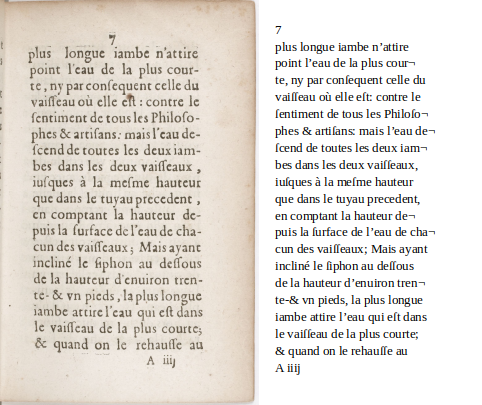
\includegraphics[scale=0.5]{pascal_15_img_transcription.png}
    \end{center} 
    \caption{Numérisation de la page 15 des \textit{Experiences Nouvelles touchant le vide…} de Pascal (1647) 
    présentée avec sa transcription diplomatique.} \label{pascal}
    \end{figure}

    Rassemblé et transcrit par \cite{Gabay2019a},
    le corpus de travail est une sélection de certaines \oe{}uvres françaises du XVII\ieme~siècle 
    décrites dans le tableau \ref{tab:corpus}. Notre corpus environ 6~000 lignes, 30~000 mots et 15~0000 caractères. 
    Un exemple de numérisation est proposé dans la figure \ref{pascal}.

    \begin{table}[h]
    \begin{center}
    \begin{footnotesize}
    {\setlength{\tabcolsep}{0.1cm}
    \begin{tabular}{|l|c|c|c|l|c|c|c|}
    \hline
    \multicolumn{4}{|c}{i)}&\multicolumn{4}{|c|}{ii)}\\\hline
    \textbf{Identifiant}&\textbf{Nb lignes}&\textbf{Nb mots}&\textbf{Nb caractères}&\textbf{Identifiant}&\textbf{Nb lignes}&\textbf{Nb mots}&\textbf{Nb caractères}\\ \hline
    Bossuet-1683&27&770&4~128&Papin-1682&23&548&2~230\\ \hline
    Chapelain-1656&28&753&4~735&Pascal-1647&39&776&3~568\\ \hline
    Ellain-1606&22&618&3~168&Sales-1641&25&618&3~915\\ \hline
    Gournay-1622&31&825&4~284&Viau-1623&33&852&4~055\\\hline
    \end{tabular}}
    \caption{Description des sous-corpus dédiés à i) l'apprentissage des modèles de langue et ii) l'océrisation
    et l'évaluation de la qualité des sorties d'OCR.} \label{tab:souscorpus}
    \end{footnotesize}
    \end{center}
    \end{table} 

    Les variétés thématique et diachronique du corpus ainsi que les transcriptions diplomatiques de grande qualité 
    permettent de le considérer non seulement comme un premier laboratoire privilégié pour l'étude 
    de l'OCR mais aussi comme représentant de cet état de langue. Ainsi les \oe{}uvres de Bossuet, Chapelin, 
    Ellain et Gournay et les \oe{}uvres de Papin, Pascal, Sales et Viau constituent-elles deux sous-corpus :
    les transcriptions des premières permettant l'apprentissage des modèles de langues et les images et 
    les transcriptions des secondes l'application des logiciels d'OCR et la mesure du \textit{CER} respectivement 
    (voir la table \ref{tab:souscorpus}).

    \subsection{Océrisation}
    Le corpus dédié à l'océrisation est composé de 120 pages numérisées, toutes avec une résolution de 400dpi. 
    Afin de réaliser l'océrisation de ces images, deux logiciels ont été utilisés :
    \begin{itemize}
      \item \verb!Kraken!, version 2.0.8\footnote{http://kraken.re/ et https://pypi.org/project/kraken/} (voir \cite{Kiessling2019a}) ;
      \item \verb!Tesseract!, version 0.3.3\footnote{https://pypi.org/project/pytesseract/} (voir \cite{Smith2007a}).
    \end{itemize}

        \paragraph{Pré-traitement des images}
        Pour appliquer ses modèles de reconnaissance de caractères, \verb!Kraken! prend en entrée des \textit{lignes}
        binarisées (un pixel ne peut être que blanc ou noir) alors que \verb!Tesseract! peut admettre des pages 
        entières en nuances de gris ou même en couleurs. Dans un souci d'unité, et puisque \verb!Kraken! est plus
        restrictif que \verb!Tesseract!, toutes les images ont été segmentées et binarisées en utilisant les modules
        dédiés de \verb!Kraken!. Ceci constitue un biais au regard des performances de \verb!Tesseract! ; néanmoins, et selon
        notre hypothèse, le taux d'erreur devrait évoluer dans le même sens que les métriques d'estimation de l'étude. 

        \paragraph{Application des modèles}
        L'objectif étant d'observer dans quelle mesure les modèles de langue peuvent être de bons indicateurs de la
        qualité d'une sortie d'OCR, l'utilisation de plusieurs modèles, adaptés ou non aux documents de l'étude,
        apparaît primordiale. Pour ce faire, les modèles de \verb!Kraken! (anglais contemporain) et de \verb!Tesseract! (français contemporain) ont été appliqués
        aux lignes segmentées et binarisées ainsi qu'un modèle \verb!Kraken! appris sur ces mêmes données\footnote{https://github.com/e-ditiones/OCR17}. 
        On dispose alors \textit{a priori} de deux modèles non adaptés aux documents de l'étude\footnote{Par exemple, le 
        <\textlongs > ne fait pas partie du vocabulaire des modèles de \verb!Kraken! (anglais) et de \verb!Tesseract! (français).} 
        et d'un modèle suradapté à ces documents (puisqu'appris sur ceux-ci). L'hypothèse que nous faisons est que 
        l'agrégation des probabilités offertes par les modèles de langue sur les sorties des modèles de 
        \verb!Kraken! et de \verb!Tesseract! sera plus faible que sur les sorties du modèle \verb!Kraken! appris sur ces 
        mêmes données. 

    \begin{table}[h]
    \begin{scriptsize}
    {\setlength{\tabcolsep}{0.15cm}
    \begin{tabular}{llllll}
    \multicolumn{1}{c}{\textbf{Lignes Kraken}} & \multicolumn{1}{l}{\textbf{CER}} & \multicolumn{1}{c}{\textbf{Lignes Tesseract}} & \multicolumn{1}{l}{\textbf{CER}} & \multicolumn{1}{c}{\textbf{Lignes Kraken 17}}                                                            & \multicolumn{1}{l}{\textbf{CER}} \\
                                               & 100 \%                           &                                               & 100 \%                           & ¬                                                                                                        & 100 \%                           \\
    plus longue iambe n'attire                 & 3,8 \%                         & plus Jongue iambe n'attire                    & 7,6 \%                         & plus longue iambe n’attire                                                                               & 0 \%                             \\
    point lcau de la plus cour-                & 7,4 \%                         & point l'eau de la plus cour-                  & 3,7 \%                         & point l’eau de la plus cour¬                                                                             & 0 \%                             \\
    te, ny par confequent celle du             & 3,4 \%                         & te, ny par confequent celle du                & 3,4 \%                         & te, ny par con\textlongs equent celle du                                                  & 0 \%                             \\
    vaifeau oi elle ef : contre le             & 16,6 \%                        & vaiffeau où elle et : contre le               & 10 \%                            & vai\textlongs \textlongs eau ou elle elt: contre le                        & 6,6 \%                         \\
    fentiment de tous les Philofo-             & 6,8 \%                         & fentiment de tous les Philofo-                & 6,8 \%                         & \textlongs entiment de tous les Philo\textlongs o¬                         & 0 \%                             \\
    phes artifans: maislcau de-                & 14,8 \%                        & phes \& artifans: mais l'eau de-              & 7,4 \%                         & phes \& arti\textlongs ans. mais l’eau de¬                                                & 0 \%                             \\
    fcend de toutes lcs dcuxiam-               & 14,2 \%                        & fcend de toutes les deuxiam-                  & 7,1 \%                         & \textlongs cend de toutes les deux iam¬                                                   & 0 \%                             \\
    bes dans les dcux vaiffeaux,               & 11,1 \%                        & bes dans les deux vaiffeaux ,                 & 7,4 \%                         & bes dans les deux vai\textlongs \textlongs eaux,                           & 0 \%                             \\
    iufques a la mefme hauteur                 & 11,5\%                        & iufques à la mefme hauteur                    & 7,6 \%                         & iu\textlongs ques à la me\textlongs me hauteur                            & 3,8 \%                         \\
    que dans le tuyau preccdent,               & 3,7 \%                         & que dans le tuyau precedent ,                 & 0 \%                             & que dans le tuyau precedent,                                                                             & 0 \%                             \\
    en comptant la hautcur dec-                & 13,6 \%                        & en comptant la hauteur de-                    & 4,5\%                          & en comptant la hauteur de¬                                                                               & 0 \%                             \\
    puis la furface deleau de cha-             & 12,9 \%                        & puis la furface de l’eau de cha-              & 6,4 \%                         & puis la \textlongs urface de l’eau de cha¬                                                & 0 \%                             \\
    cun des vaiffcaux; Mais ayant              & 10,7 \%                        & cun des vaiffeaux; Maisayant                  & 10,7 \%                        & cun des vai\textlongs \textlongs eaux; Mais ayant                          & 0 \%                             \\
    inclin lc fiphon au deffous                & 17,8 \%                        & incliné le fiphon au deffous                  & 10,7 \%                        & incliné le \textlongs iphon au de\textlongs \textlongs ous & 3,7 \%                         \\
    dc la hautcur dcnuiron trcn-               & 17,8 \%                        & de la hauteur d'enuiron tren-                 & 3,5 \%                         & de la hauteur d’enuiron tren¬                                                                            & 0 \%                             \\
    te- vn picds, lapluslongue                 & 11,5 \%                        & te- \& vn picds, la plus longue               & 3,8 \%                         & te \& vn pieds, la plus longue                                                                           & 0 \%                             \\
    iambe attirclcau qui eft dans              & 16,1 \%                        & jambe attire l'eau qui eft dans               & 9,6 \%                         & iambe attire l’eau qui e\textlongs t dans                                                 & 0 \%                             \\
    le vaifeau de la plus courte;              & 6,8 \%                         & le vaiffeau de la plus courtc;                & 10,3 \%                        & e vai\textlongs \textlongs eau de la plus courte;                          & 3,4 \%                         \\
    quand on le rehaufe au                     & 8,6 \%                         & \& quand on le rehaufle au                    & 8,6 \%                         & \& quand on le rehau\textlongs \textlongs e au                             & 0 \%                             \\
    A iii                                      & 16,6 \%                        & À ill                                         & 66,6 \%                        & A iii                                                                                                    & 16,6 \%                       
    \end{tabular}}\cprotect\caption{Sorties des trois modèles d'OCR pour la 15\ieme~page des \textit{Experiences Nouvelles touchant le vide…} de Pascal (1647).
        De gauche à droite : modèle \verb!Kraken! (anglais), modèle \verb!Tesseract! (français) et modèle \verb!Kraken! (français du XVII\ieme~siècle).} \label{ocr}
    \end{scriptsize}
    \end{table}

    Le tableau \ref{ocr} présente un exemple des sorties des trois modèles d'OCR sélectionnés.

    \subsection{Apprentissage des modèles de langue}
    Deux types de modèles de langue (au grain caractère) ont été appris sur le sous-corpus dédié (voir la table \ref{tab:souscorpus})
    qui compte 121 caractères différents :
    \begin{itemize}
      \item des modèles de langue à probabilités conditionnelles, appris comme la probabilité d'observer un caractère 
      sachant une séquence de caractères (un historique) ;
      \item des modèles de langue appris par des réseaux de neurones (LSTM et biLSTM).
    \end{itemize}
    Les premiers types de modèles sont construits en comptant, 
    par fenêtre glissante sur le corpus d'apprentissage, le nombre d'occurrences du caractère suivant
    la séquence de caractères contenue dans la fenêtre glissante. Ces occurrences absolues sont ensuite 
    divisées par la somme des occurrences de tous les caractères suivants cette séquence et sont utilisées
    comme des probabilités, puisque contenues dans l'intervalle $\left[0;1\right]$. Les seconds sont appris
    en utilisant les modèles séquentiels de la librairie Python \textit{keras}. Un \textit{mapping} du vocabulaire
    est d'abord réalisé en prétraitement\footnote{\`{A} chaque élément du vocabulaire (entendu comme l'ensemble des caractères 
    différents) est associé un entier dans une table.}. Les réseaux LSTM et biLSTM contiennent tous une couche 
    \textit{LSTM} et aux réseaux biLSTM est ajoutée une couche \textit{Bidirectional}. La fonction \textit{softmax} est 
    enfin utilisée comme fonction d'activation. Ces modèles de langue ont été appris sur des séquences de \textit{n} 
    caractères, pour \textit{n} variant de 2 à 10. Finalement, on dispose donc de $3 * 9 = 27$ modèles de langue
    pour tester l'estimation de la qualité des sorties des logiciels d'OCR. Le nombre de caractères dans le vocabulaire de ces
    modèles de langue est de 121.

    \subsection{Métriques d'estimation}\label{metric}

    	\subsubsection{Préambules} 

	    	\paragraph{Calcul du \textit{CER}}
	    	Le \textit{CER} est calculé entre une suite de caractères de référence et une suite à tester comme la somme des 
	        insertions, délétions et substitutions divisée par le nombre total de caractères de la chaîne de référence. 
	        Il peut être supérieur à 1 si le nombre d'insertions est particulièrement élevé.

	        \paragraph{Probabilités des modèles de langue}\label{probaLM}
			Les modèles de langue permettent de disposer de la probabilité qu'un caractère donné suive une certaine séquence de 
		    caractères. Si une sortie de logiciel d'OCR est parcourue par une fenêtre glissante à partir de laquelle est renvoyée une
		    séquence de caractères et le caractère suivant cette séquence, pour une sortie d'OCR on dispose d'une suite d'au plus
		    $C - n$ probabilités, avec $C$ le nombre total de caractères et $n$ la taille de la fenêtre glissante en caractères.
		    \textit{Au plus} car il est possible que certains caractères fournis par le modèle d'OCR n'aient pas été rencontrés
		    dans le corpus d'apprentissage du modèle de langue\footnote{Par exemple,  \verb!Kraken! (anglais) et 
		    \verb!Tesseract! (français), appris sur des documents contemporains, ont dans leur vocabulaire le symbole \euro{} et peuvent le proposer
		    dans leur océrisation. Pour un modèle de langue appris sur des données textuelles françaises du XVII\ieme~siècle,
		    ce symbole n'existe pas.}. 

	    	On cherche donc à agréger ces probabilités, pour chaque document du corpus océrisé, dans l'objectif que ces agrégats
	    	soient corrélés au \textit{CER} qu'on peut calculer grâce aux transcriptions. Il s'agit de calculer d'autres métriques
	    	ne nécessitant pas de vérité de terrain (à partir des probabilités fournies par les modèles de langue) et de valider ou
	    	réfuter la pertinence de leur estimation de la qualité d'une sortie d'OCR face à une métrique de référence, le \textit{CER}.

        
	   \subsubsection{Agrégations des probabilités des modèles de langue}\label{metrics}
	       \paragraph{La somme des probabilités}
	       Une première métrique peut être simplement la somme des probabilités renvoyées par les modèles de langue. Pour une
	       sortie d'OCR, on a donc : 
	       $$S = \sum_{i=n+1}^{C-n}P_{LM}(c_{i} | h_{n,i})$$
	       Avec $P_{LM}$ la probabilité renvoyée par un modèle de langue $LM$, $n$ 
	       la taille de la fenêtre glissante en caractères, $C$ le nombre total de caractères de la sortie d'OCR, $c_{i}$ 
	       le $i$\ieme~caractère de la sortie d'OCR et $h_{n,i}$ l'historique de $n$ caractères du caractère $c_{i}$.

	       \paragraph{Le produit des probabilités}
	       De la même manière, le produit des probabilités peut constituer une autre métrique d'estimation. Il est défini
	       comme :
	       $$Pr = \prod_{i=n+1}^{C-n}P_{LM}(c_{i} | h_{n,i})$$

	       \paragraph{La perplexité}
	       Plus couramment utilisée pour juger de la qualité d'un modèle de langue, la perplexité est la probabilité inverse de la sortie
	       d'OCR normalisée par son nombre de caractères. Elle est définie comme : 
	        $$PP = \frac{1}{(\prod_{i=n+1}^{C-n}P_{LM}(c_{i} | h_{n,i}))^{\frac{1}{C-n}}}$$

	       \paragraph{La log-perplexité}
	       $$log(PP)$$

	    \subsubsection{\'{E}chelles de calcul des agrégations}\label{echelle}
	    Les agrégations des probabilités précitées peuvent être calculées à plusieurs échelles : celle de l'\oe{}uvre, de la page, de la ligne 
	    ou encore du mot. Puisque la perplexité $PP$ est calculée comme l'inverse d'une racine $n$-ième, elle tend vers 1 à mesure que le nombre 
	    total de caractères $C - n$ grandit. Plus le nombre de caractères sur lesquels elle est calculée grandit, moins elle est informative. 
	    Les estimateurs de qualité d'océrisation des pages sont donc calculés comme la moyenne des agrégations des probabilités
	    calculées à l'échelle du mot\footnote{La tokenisation est réalisée par une simple segmentation par l'espace des chaînes de caractères.}.

	    Notons que réaliser une \textit{moyenne} constitue un bais important. Les données textuelles issues d'OCR n'ont pas une qualité homogène
	    pour une même \oe{}uvre ou une même page ; la moyenne efface ces disparités pourtant essentielles à soulever. D'autre
	    part, certains mots comportent trop peu de caractères pour que le modèle de langue puisse leur calculer une probabilité. Certains passages sont 
	    ignorés et la moyenne ne le traduit pas. 


\section{Expérimentations et résultats}\label{expe}

Pour calculer les métriques d'estimation de la qualité de l'OCR sur une page du corpus, on calcule ces métriques pour chaque mot de la page
et on en fait la moyenne. Afin de confirmer ou réfuter l'intérêt de ces métriques, un calcul de corrélation 
Pearson\footnote{En tant que normalisation des covariances, le coefficient de corrélation exprime à quel point deux variables 
sont liées. Ce coefficient étant une normalisation, il appartient à l'intervalle $\left[-1;1\right]$ ; les corrélations 
positives indiquent que les deux variables évoluent dans le même sens et les corrélations négatives qu'elles évoluent dans un sens opposé. 
Plus une corrélation est proche de $1$ ou $-1$, plus le lien entre les deux variables est fort ; au
contraire, plus la corrélation est proche de $0$, plus ce lien se dissipe. Notons finalement qu'une corrélation n'est 
significative que pour une $p$-$value < 0,05$.}  
est réalisé avec le \textit{CER}. Si une ou plusieurs métriques est corrélée-s significativement au \textit{CER}, on peut
conclure que l'apprentissage d'un modèle de langue sur des données du français du XVII\ieme~siècle et l'utilisation de ses 
probabilités pour estimer la qualité d'une sortie d'OCR sur des documents de la même période sont justifiés.

    \subsection{Préambule à l'analyse des corrélations}
    
        \begin{table}[h]
        \begin{center}
        \begin{tabular}{|l|c|c|c|}
        \hline
        \textbf{Métriques}  & \textbf{Variations} & \textbf{Signes des corrélations avec le \textit{CER}}    \\\hline
        $CER$  & $\nearrow$      &     \\ 
        $S$    & $\searrow$     & -   \\ 
        $Pr$    & $\searrow$     & -   \\
        $Pr^\frac{1}{C-n}$   & $\searrow$    & -    \\
        $PP=\frac{1}{Pr ^{\frac{1}{C-n}}}$ & $\nearrow$   & +   \\ 
        $\log \left (   PP   \right )$  & $\nearrow$      & + \\ 
        \hline
        \end{tabular}
        \caption{Variations et signes des corrélations avec le \textit{CER} des métriques d'estimation pour un nombre d'erreurs qui augmente.} \label{tab:var_cor}
        \end{center}
        \end{table}

    Le tableau \ref{tab:var_cor} expose la variation des métriques d'estimation et le signe de leur 
    corrélation avec le \textit{CER} pour un nombre d'erreurs d'océrisation qui augmente. L'hypothèse est que les
    modèles de langue fournissent des probabilités (voir le paragraphe \ref{probaLM})
    plus élevées face à une sortie d'OCR sans erreur (du \textit{texte}) et des
    probabilités plus faibles face à une sortie d'OCR avec erreurs (du \textit{non-texte}). Ainsi, pour valider les métriques comme estimateurs pertinents, les corrélations entre le \textit{CER} et la somme et le produit des 
    probabilités doivent être négatives alors qu'elles doivent être positives entre le \textit{CER}
    et la perplexité et la log-perplexité.
    


    \subsection{Corrélations entre le \textit{CER} et les métriques d'estimation}
    \begin{table}
    \begin{center}
    \begin{scriptsize}
    
    \begin{tabular}{|l|c|c|c|c|c|c|c|c|}

    \multicolumn{9}{c}{{\footnotesize Modèle par défaut de Kraken. Modèles de langue à probabilités conditionnelles (\textit{n} variant de 2 à 10).}}\\\hline
    \multirow{2}{*}{\textbf{}} & \multicolumn{2}{c|}{\textbf{S}}         & \multicolumn{2}{c|}{\textbf{Pr}}        & \multicolumn{2}{c|}{\textbf{PP}}        & \multicolumn{2}{c|}{\textbf{log(PP)}}   \\ 
    \cline{2-9} & \textbf{corrélation} & \textbf{p-value} & \textbf{corrélation} & \textbf{p-value} & \textbf{corrélation} & \textbf{p-value} & \textbf{corrélation} & \textbf{p-value} \\ \hline
    
    \textbf{n=2}  & -0,063 & 0,496 & 0,111  & 0,226 & -0,016 & 0,862 & -0,013 & 0,884 \\ \hline
    \textbf{n=3}  & -0,098 & 0,287 & 0,073  & 0,426 & 0,005  & 0,955 & 0,021  & 0,820 \\ \hline
    \textbf{n=4}  & -0,073 & 0,428 & -0,043 & 0,642 & -0,010 & 0,913 & -0,014 & 0,879 \\ \hline
    \textbf{n=5}  & -0,137 & 0,135 & -0,043 & 0,638 & -0,015 & 0,868 & -0,026 & 0,780 \\ \hline
    \textbf{n=6}  & -0,093 & 0,314 & 0,000  & 0,996 & 0,067  & 0,466 & 0,059  & 0,522 \\ \hline
    \textbf{n=7}  & -0,035 & 0,708 & -0,032 & 0,728 & 0,130  & 0,157 & 0,117  & 0,205 \\ \hline
    \textbf{n=8}  & -0,064 & 0,485 & -0,074 & 0,420 & 0,043  & 0,643 & 0,054  & 0,560 \\ \hline
    \textbf{n=9}  & -0,057 & 0,538 & -0,012 & 0,898 & 0,018  & 0,846 & 0,021  & 0,821 \\ \hline
    \textbf{n=10} & -0,046 & 0,615 & -0,023 & 0,806 & 0,024  & 0,794 & 0,026  & 0,780 \\ \hline
    \end{tabular}

    \begin{tabular}{|l|c|c|c|c|c|c|c|c|}
    \multicolumn{9}{c}{{\footnotesize Modèle par défaut de Tesseract. Modèles de langue à probabilités conditionnelles (\textit{n} variant de 2 à 10).}}\\\hline
    \multirow{2}{*}{\textbf{}} & \multicolumn{2}{c|}{\textbf{S}}         & \multicolumn{2}{c|}{\textbf{Pr}}        & \multicolumn{2}{c|}{\textbf{PP}}        & \multicolumn{2}{c|}{\textbf{log(PP)}}   \\ 
    \cline{2-9} & \textbf{corrélation} & \textbf{p-value} & \textbf{corrélation} & \textbf{p-value} & \textbf{corrélation} & \textbf{p-value} & \textbf{corrélation} & \textbf{p-value} \\ \hline
    
    \textbf{n=2}  & -0,004 & 0,968 & 0,158  & 0,086          & 0,113  & 0,221          & 0,006  & 0,952          \\ \hline
    \textbf{n=3}  & -0,130 & 0,156 & 0,009  & 0,920          & -0,003 & 0,976          & 0,056  & 0,540          \\ \hline
    \textbf{n=4}  & -0,124 & 0,178 & -0,005 & 0,960          & 0,016  & 0,866          & 0,060  & 0,518          \\ \hline
    \textbf{n=5}  & -0,158 & 0,084 & -0,070 & 0,449          & 0,134  & 0,143          & 0,158  & 0,085          \\ \hline
    \textbf{n=6}  & -0,138 & 0,133 & -0,054 & 0,556          & 0,180  & \textbf{0,049} & 0,188  & \textbf{0,040} \\ \hline
    \textbf{n=7}  & -0,100 & 0,278 & -0,027 & 0,773          & 0,093  & 0,313          & 0,084  & 0,359          \\ \hline
    \textbf{n=8}  & -0,055 & 0,547 & -0,008 & 0,930          & -0,006 & 0,949          & -0,008 & 0,928          \\ \hline
    \textbf{n=9}  & -0,054 & 0,554 & -0,083 & 0,366          & 0,096  & 0,299          & 0,095  & 0,300          \\ \hline
    \textbf{n=10} & -0,024 & 0,796 & -0,212 & \textbf{0,020} & 0,228  & \textbf{0,012} & 0,187  & \textbf{0,041} \\ \hline
    
    \end{tabular}
    \begin{tabular}{|l|c|c|c|c|c|c|c|c|}

    \multicolumn{9}{c}{{\footnotesize Modèle Kraken XVII\ieme~siècle. Modèles de langue à probabilités conditionnelles (\textit{n} variant de 2 à 10).}}\\\hline
    \multirow{2}{*}{\textbf{}} & \multicolumn{2}{c|}{\textbf{S}}         & \multicolumn{2}{c|}{\textbf{Pr}}        & \multicolumn{2}{c|}{\textbf{PP}}        & \multicolumn{2}{c|}{\textbf{log(PP)}}   \\ 
    \cline{2-9} & \textbf{corrélation} & \textbf{p-value} & \textbf{corrélation} & \textbf{p-value} & \textbf{corrélation} & \textbf{p-value} & \textbf{corrélation} & \textbf{p-value} \\ \hline

    \textbf{n=2}  & -0,052 & 0,572 & 0,129  & 0,162 & 0,238  & \textbf{0,009} & 0,040  & 0,663 \\ \hline
    \textbf{n=3}  & -0,080 & 0,384 & 0,087  & 0,343 & -0,003 & 0,970          & 0,030  & 0,742 \\ \hline
    \textbf{n=4}  & -0,041 & 0,654 & -0,010 & 0,916 & 0,012  & 0,894          & 0,031  & 0,739 \\ \hline
    \textbf{n=5}  & -0,111 & 0,225 & -0,072 & 0,437 & 0,039  & 0,670          & 0,069  & 0,452 \\ \hline
    \textbf{n=6}  & -0,135 & 0,142 & -0,055 & 0,551 & 0,138  & 0,133          & 0,143  & 0,120 \\ \hline
    \textbf{n=7}  & -0,086 & 0,348 & -0,030 & 0,746 & 0,063  & 0,496          & 0,075  & 0,414 \\ \hline
    \textbf{n=8}  & -0,096 & 0,296 & -0,030 & 0,743 & -0,045 & 0,622          & -0,045 & 0,625 \\ \hline
    \textbf{n=9}  & -0,052 & 0,574 & -0,017 & 0,857 & -0,015 & 0,874          & -0,029 & 0,757 \\ \hline
    \textbf{n=10} & -0,021 & 0,817 & -0,039 & 0,669 & 0,121  & 0,189          & 0,097  & 0,291 \\ \hline

    
    \end{tabular}
    \begin{tabular}{|l|c|c|c|c|c|c|c|c|}

    \multicolumn{9}{c}{{\footnotesize Modèle par défaut de Kraken. Modèles de langue LSTM (\textit{n} variant de 2 à 10).}}\\\hline
    \multirow{2}{*}{\textbf{}} & \multicolumn{2}{c|}{\textbf{S}}         & \multicolumn{2}{c|}{\textbf{Pr}}        & \multicolumn{2}{c|}{\textbf{PP}}        & \multicolumn{2}{c|}{\textbf{log(PP)}}   \\ 
    \cline{2-9} & \textbf{corrélation} & \textbf{p-value} & \textbf{corrélation} & \textbf{p-value} & \textbf{corrélation} & \textbf{p-value} & \textbf{corrélation} & \textbf{p-value} \\ \hline

    \textbf{n=2}  & -0,059 & 0,520          & 0,094  & 0,305          & 0,046  & 0,615 & 0,000  & 0,999 \\ \hline
    \textbf{n=3}  & -0,078 & 0,395          & 0,078  & 0,397          & -0,031 & 0,739 & -0,011 & 0,902 \\ \hline
    \textbf{n=4}  & -0,094 & 0,306          & -0,070 & 0,446          & 0,113  & 0,221 & -0,111 & 0,227 \\ \hline
    \textbf{n=5}  & -0,108 & 0,240          & -0,048 & 0,600          & -0,061 & 0,511 & -0,077 & 0,404 \\ \hline
    \textbf{n=6}  & -0,039 & 0,675          & 0,184  & \textbf{0,045} & 0,055  & 0,552 & -0,092 & 0,320 \\ \hline
    \textbf{n=7}  & 0,198  & \textbf{0,030} & -0,049 & 0,595          & -0,051 & 0,578 & 0,035  & 0,702 \\ \hline
    \textbf{n=8}  & -0,034 & 0,709          & 0,026  & 0,781          & -0,017 & 0,854 & 0,058  & 0,530 \\ \hline
    \textbf{n=9}  & -0,055 & 0,549          & -0,016 & 0,860          & -0,062 & 0,499 & 0,076  & 0,407 \\ \hline
    \textbf{n=10} & 0,063  & 0,492          & -0,036 & 0,695          & -0,055 & 0,550 & -0,061 & 0,506 \\ \hline
    
    \end{tabular}
    \begin{tabular}{|l|c|c|c|c|c|c|c|c|}

    
    
    \multicolumn{9}{c}{{\footnotesize Modèle par défaut de Tesseract. Modèles de langue LSTM (\textit{n} variant de 2 à 10).}}\\\hline
    \multirow{2}{*}{\textbf{}} & \multicolumn{2}{c|}{\textbf{S}}         & \multicolumn{2}{c|}{\textbf{Pr}}        & \multicolumn{2}{c|}{\textbf{PP}}        & \multicolumn{2}{c|}{\textbf{log(PP)}}   \\ \cline{2-9} 
                               & \textbf{corrélation} & \textbf{p-value} & \textbf{corrélation} & \textbf{p-value} & \textbf{corrélation} & \textbf{p-value} & \textbf{corrélation} & \textbf{p-value} \\ \hline
    \textbf{n=2}  & -0,010 & 0,911 & 0,138  & 0,131 & -0,032 & 0,730 & -0,081 & 0,377 \\ \hline
    \textbf{n=3}  & -0,132 & 0,151 & -0,046 & 0,621 & -0,004 & 0,962 & 0,133  & 0,148 \\ \hline
    \textbf{n=4}  & -0,085 & 0,354 & -0,053 & 0,567 & 0,003  & 0,972 & -0,009 & 0,926 \\ \hline
    \textbf{n=5}  & -0,096 & 0,298 & -0,080 & 0,383 & -0,022 & 0,808 & 0,053  & 0,568 \\ \hline
    \textbf{n=6}  & -0,107 & 0,245 & 0,034  & 0,716 & -0,010 & 0,915 & -0,038 & 0,683 \\ \hline
    \textbf{n=7}  & -0,116 & 0,208 & -0,079 & 0,390 & 0,106  & 0,250 & 0,007  & 0,938 \\ \hline
    \textbf{n=8}  & 0,043  & 0,640 & -0,026 & 0,776 & -0,034 & 0,711 & -0,025 & 0,788 \\ \hline
    \textbf{n=9}  & -0,044 & 0,636 & 0,024  & 0,791 & -0,032 & 0,732 & 0,029  & 0,756 \\ \hline
    \textbf{n=10} & -0,025 & 0,788 & -0,072 & 0,432 & 0,012  & 0,895 & 0,073  & 0,426 \\ \hline
    
\end{tabular}
    \end{scriptsize}\end{center}\end{table}


    \begin{table}
    \begin{center}
    \begin{scriptsize}
    
    \begin{tabular}{|l|c|c|c|c|c|c|c|c|}
    

    
    \multicolumn{9}{c}{{\footnotesize Modèle Kraken XVII\ieme~siècle. Modèles de langue LSTM (\textit{n} variant de 2 à 10).}}\\\hline
    \multirow{2}{*}{\textbf{}} & \multicolumn{2}{c|}{\textbf{S}}         & \multicolumn{2}{c|}{\textbf{Pr}}        & \multicolumn{2}{c|}{\textbf{PP}}        & \multicolumn{2}{c|}{\textbf{log(PP)}}   \\ \cline{2-9} 
                               & \textbf{corrélation} & \textbf{p-value} & \textbf{corrélation} & \textbf{p-value} & \textbf{corrélation} & \textbf{p-value} & \textbf{corrélation} & \textbf{p-value} \\ \hline
    \textbf{n=2}  & -0,055 & 0,552          & 0,168  & 0,066 & -0,006 & 0,944 & -0,049 & 0,596 \\ \hline
    \textbf{n=3}  & -0,065 & 0,482          & 0,114  & 0,215 & -0,023 & 0,804 & -0,062 & 0,503 \\ \hline
    \textbf{n=4}  & -0,058 & 0,526          & -0,030 & 0,741 & -0,026 & 0,777 & -0,024 & 0,793 \\ \hline
    \textbf{n=5}  & -0,069 & 0,455          & -0,052 & 0,576 & -0,012 & 0,898 & -0,005 & 0,953 \\ \hline
    \textbf{n=6}  & -0,083 & 0,366          & 0,045  & 0,623 & -0,008 & 0,930 & 0,017  & 0,856 \\ \hline
    \textbf{n=7}  & -0,067 & 0,465          & -0,049 & 0,595 & -0,027 & 0,773 & -0,056 & 0,541 \\ \hline
    \textbf{n=8}  & -0,104 & 0,258          & -0,041 & 0,653 & -0,030 & 0,745 & -0,029 & 0,751 \\ \hline
    \textbf{n=9}  & -0,023 & 0,805          & -0,036 & 0,697 & -0,022 & 0,809 & -0,034 & 0,710 \\ \hline
    \textbf{n=10} & 0,181  & \textbf{0,048} & -0,059 & 0,520 & -0,006 & 0,947 & -0,012 & 0,898 \\ \hline
     



    \end{tabular}
    \begin{tabular}{|l|c|c|c|c|c|c|c|c|}
    \multicolumn{9}{c}{{\footnotesize Modèle par défaut de Kraken. Modèles de langue biLSTM (\textit{n} variant de 2 à 10).}}\\\hline
    \multirow{2}{*}{\textbf{}} & \multicolumn{2}{c|}{\textbf{S}}         & \multicolumn{2}{c|}{\textbf{Pr}}        & \multicolumn{2}{c|}{\textbf{PP}}        & \multicolumn{2}{c|}{\textbf{log(PP)}}   \\ \cline{2-9} 
                               & \textbf{corrélation} & \textbf{p-value} & \textbf{corrélation} & \textbf{p-value} & \textbf{corrélation} & \textbf{p-value} & \textbf{corrélation} & \textbf{p-value} \\ \hline
    \textbf{n=2}  & -0,042 & 0,645 & 0,115  & 0,213 & -0,040 & 0,661          & -0,043 & 0,641 \\ \hline
    \textbf{n=3}  & -0,098 & 0,289 & 0,160  & 0,081 & -0,096 & 0,295          & -0,077 & 0,404 \\ \hline
    \textbf{n=4}  & -0,091 & 0,320 & -0,087 & 0,346 & 0,085  & 0,357          & -0,126 & 0,170 \\ \hline
    \textbf{n=5}  & -0,019 & 0,837 & -0,085 & 0,354 & -0,049 & 0,595          & -0,013 & 0,891 \\ \hline
    \textbf{n=6}  & -0,076 & 0,411 & 0,131  & 0,154 & -0,040 & 0,662          & -0,087 & 0,345 \\ \hline
    \textbf{n=7}  & 0,010  & 0,914 & -0,105 & 0,255 & -0,058 & 0,529          & 0,009  & 0,925 \\ \hline
    \textbf{n=8}  & -0,053 & 0,564 & -0,085 & 0,357 & 0,623  & \textbf{0,001} & 0,053  & 0,563 \\ \hline
    \textbf{n=9}  & -0,070 & 0,446 & -0,060 & 0,517 & -0,024 & 0,794          & -0,054 & 0,560 \\ \hline
    \textbf{n=10} & 0,084  & 0,361 & -0,028 & 0,758 & -0,033 & 0,722          & -0,059 & 0,521 \\ \hline
    



    \end{tabular}
    \begin{tabular}{|l|c|c|c|c|c|c|c|c|}
    \multicolumn{9}{c}{{\footnotesize Modèle par défaut de Tesseract. Modèles de langue biLSTM (\textit{n} variant de 2 à 10).}}\\\hline
    \multirow{2}{*}{\textbf{}} & \multicolumn{2}{c|}{\textbf{S}}         & \multicolumn{2}{c|}{\textbf{Pr}}        & \multicolumn{2}{c|}{\textbf{PP}}        & \multicolumn{2}{c|}{\textbf{log(PP)}}   \\ \cline{2-9} 
                               & \textbf{corrélation} & \textbf{p-value} & \textbf{corrélation} & \textbf{p-value} & \textbf{corrélation} & \textbf{p-value} & \textbf{corrélation} & \textbf{p-value} \\ \hline
    \textbf{n=2}  & 0,013  & 0,886 & 0,184  & \textbf{0,044} & 0,000  & 1,000 & -0,117 & 0,203 \\ \hline
    \textbf{n=3}  & -0,137 & 0,137 & -0,022 & 0,816          & 0,117  & 0,203 & 0,157  & 0,087 \\ \hline
    \textbf{n=4}  & -0,040 & 0,663 & 0,011  & 0,909          & -0,025 & 0,788 & -0,051 & 0,577 \\ \hline
    \textbf{n=5}  & -0,079 & 0,389 & -0,055 & 0,547          & -0,006 & 0,946 & 0,023  & 0,800 \\ \hline
    \textbf{n=6}  & -0,058 & 0,530 & -0,012 & 0,893          & -0,045 & 0,627 & -0,098 & 0,287 \\ \hline
    \textbf{n=7}  & -0,064 & 0,485 & -0,013 & 0,885          & -0,007 & 0,943 & -0,093 & 0,314 \\ \hline
    \textbf{n=8}  & 0,036  & 0,696 & -0,023 & 0,801          & 0,051  & 0,580 & -0,036 & 0,694 \\ \hline
    \textbf{n=9}  & -0,053 & 0,566 & -0,033 & 0,724          & 0,007  & 0,936 & 0,050  & 0,586 \\ \hline
    \textbf{n=10} & -0,029 & 0,754 & 0,029  & 0,756          & -0,024 & 0,797 & 0,027  & 0,773 \\ \hline



    \end{tabular}
    \begin{tabular}{|l|c|c|c|c|c|c|c|c|}
    \multicolumn{9}{c}{{\footnotesize Modèle Kraken XVII\ieme~siècle. Modèles de langue biLSTM (\textit{n} variant de 2 à 10).}}\\\hline
    \multirow{2}{*}{\textbf{}} & \multicolumn{2}{c|}{\textbf{S}}         & \multicolumn{2}{c|}{\textbf{Pr}}        & \multicolumn{2}{c|}{\textbf{PP}}        & \multicolumn{2}{c|}{\textbf{log(PP)}}   \\ \cline{2-9} 
                               & \textbf{corrélation} & \textbf{p-value} & \textbf{corrélation} & \textbf{p-value} & \textbf{corrélation} & \textbf{p-value} & \textbf{corrélation} & \textbf{p-value} \\ \hline
    \textbf{n=2}  & -0,061 & 0,508          & 0,146  & 0,113 & 0,002  & 0,985 & -0,060 & 0,513 \\ \hline
    \textbf{n=3}  & -0,075 & 0,413          & 0,101  & 0,273 & -0,026 & 0,779 & -0,111 & 0,228 \\ \hline
    \textbf{n=4}  & -0,048 & 0,601          & -0,045 & 0,622 & -0,011 & 0,909 & -0,078 & 0,396 \\ \hline
    \textbf{n=5}  & -0,040 & 0,661          & -0,106 & 0,250 & -0,038 & 0,681 & -0,014 & 0,878 \\ \hline
    \textbf{n=6}  & -0,045 & 0,622          & -0,010 & 0,917 & -0,048 & 0,605 & -0,041 & 0,660 \\ \hline
    \textbf{n=7}  & -0,106 & 0,251          & 0,064  & 0,489 & -0,005 & 0,955 & -0,021 & 0,823 \\ \hline
    \textbf{n=8}  & -0,086 & 0,350          & -0,057 & 0,539 & 0,022  & 0,815 & -0,076 & 0,410 \\ \hline
    \textbf{n=9}  & -0,017 & 0,855          & -0,033 & 0,721 & -0,007 & 0,940 & 0,011  & 0,908 \\ \hline
    \textbf{n=10} & 0,202  & \textbf{0,027} & -0,025 & 0,786 & -0,027 & 0,767 & 0,012  & 0,898 \\ \hline


    \end{tabular} \cprotect\caption{Corrélations et \textit{p-values} calculées entre les métriques d'estimation et le \textit{CER}. Modèles d'OCR : modèles \verb!Kraken! (anglais), \verb!Tesseract! (français) et modèle \verb!Kraken! (français du XVII\ieme~siècle). Types de modèles de langue : probabilités conditionnelles, LSTM et biLSTM.}\label{tab:res_corr}
    \end{scriptsize}
    \end{center}   
    \end{table}
   

    Le sous-corpus dédié à l'OCR est composé de 118 pages.
    On peut donc, pour les sorties des trois modèles d'OCR utilisés et pour les trois types de modèles de langue, calculer 
    les métriques d'estimation et le \textit{CER}, et ce pour chaque page du corpus. 

    Le tableau \ref{tab:res_corr} montre des \textit{p-values} presque toutes supérieures à $0,05$, ce qui signifie que s'il y a
    corrélation, elle n'est pas significative. Ces résultats semblent réfuter l'hypothèse initiale selon laquelle les probabilités 
    des modèles de langue auraient pu être agrégées pour se substituer à un \textit{CER} exigeant une vérité de terrain. 

    \subsection{Les modèles de langue sont-ils inadaptés ?}

    \begin{table}[h]
    \begin{footnotesize}
    \begin{center}
    \begin{tabular}{|l|c|c|c|}
    \hline
                  & \textbf{ML probabilités conditionnelles} & \multicolumn{1}{r|}{\textbf{ML LSTM}} & \textbf{ML biLSTM} \\ \hline
    \textbf{n=2}  & 90                                       & 14721                                 & 257646757092       \\ \hline
    \textbf{n=3}  & 126                                      & 1010690                               & 235913940342       \\ \hline
    \textbf{n=4}  & 426                                      & 318251055                             & 221055920422       \\ \hline
    \textbf{n=5}  & 1091                                     & 723946838                             & 211044617070       \\ \hline
    \textbf{n=6}  & 1978                                     & 690749546                             & 204520506752       \\ \hline
    \textbf{n=7}  & 2801                                     & 669397958                             & 200184237186       \\ \hline
    \textbf{n=8}  & 3510                                     & 655634987                             & 1161841181775      \\ \hline
    \textbf{n=9}  & 3940                                     & 647905538                             & 13807745026062     \\ \hline
    \textbf{n=10} & 4205                                     & 643364471                             & 14481238375005     \\ \hline
    \end{tabular}\caption{Moyennes des perplexités des modèles de langue sur le sous-corpus de test.}\label{tab:perplex}
    \end{center}
    \end{footnotesize}
    \end{table}


    Les résultats précédents suggèrent que i) soit les modèles de langue sont de mauvaise qualité, ii) soit le corpus de l'étude présente des spécificités particulières 
    ou iii) soit les deux raisons précitées concourent à cette impasse.

    Les modèles de langue ont été appris sur les \oe{}uvres de Bossuet, Chapelin, Ellain et Gournay. On peut donc les
    évaluer en calculant leur perplexité sur le sous-corpus des \oe{}uvres de Papin, Pascal, Sales et Viau. 
    Le tableau \ref{tab:perplex} présente les moyennes des perplexités des modèles de langue
    de l'étude calculées sur les vérités de terrain. Les modèles de langue LSTM et biLSTM 
    présentent des perplexités aberrantes (ils sont non adaptés à la tâche) alors que seuls les modèles de langue à probabilités conditionnelles, pour $n \in \left[2;4\right]$,
    présentent une meilleure qualité. Nous concluons donc que la mauvaise qualité des modèles de langue
    explique la non corrélation entre les estimateurs et le \textit{CER}.



    


\section{Conclusion}
La mauvaise qualité des modèles de langue ne permet pas de valider ou réfuter notre hypothèse, selon laquelle agréger les 
probabilités des modèles de langue permettrait d'estimer la qualité d'une sortie d'OCR. Pour en faire l'expérience, il s'agirait 
de renouveler ces tests avec un ensemble plus vaste de transcriptions d'imprimés du XVII\ieme~siècle. Nous cherchions à proposer une 
alternative au manque de vérités de terrain mais nous constatons qu'un ensemble de 108 pages (16~315 mots) est insuffisant. 
Si cela ne contredit pas l'éventuelle pertinence des estimateurs envisagés, un ensemble conséquent de données textuelles en français du 
XVII\ieme~siècle reste nécessaire au bon apprentissage des modèles langue. Nous rassemblerons donc plus de données textuelles en 
français du XVII\ieme~siècle pour reconduire l'expérience avec des modèles de langue de meilleure qualité. 


Les programmes, en Python 3.7, sont mis à disposition sur : \url{https://github.com/anonyme}.

\section*{Remerciements}
Ce travail n'aurait pas été possible sans l'aide de Simon Gabay, Gaël Lejeune et Alice Millour.  

\bibliographystyle{jeptaln2020}
\bibliography{historical_documents_OCR.bib}
\nocite{Wick2018a, Springmann2016b, BergKirkpatrick2014a,Breuel2013a,Vamvakas2008a}



%%================================================================
\end{document}
